% --- Use Case U3.1 ---
\subsubsection{Use-case U3.1: Xem lịch sử giao dịch cá nhân}
\vspace{0.5cm}
\noindent
\begin{tabularx}{\textwidth}{|>{\raggedright\arraybackslash}p{4cm}|X|}
\hline
\textbf{Use-case ID} \newline \textbf{Use-case name} & U3.1 \newline \textbf{Xem lịch sử giao dịch cá nhân
} \\ \hline
\textbf{Use-case overview} & Cho phép người dùng xem toàn bộ lịch sử giao dịch. \\ \hline
\textbf{Actors} & 1. Khách gửi xe có tài khoản \\  \hline
\textbf{Preconditions} & 
1. Hệ thống kết nối tới các máy chủ đã xác thực và khả dụng.\newline
2. Người dùng đã đăng nhập vào hệ thống.\\ \hline
\textbf{Trigger} & Người dùng chọn “Lịch sử giao dịch”. \\ \hline
\textbf{Steps} & 
1. Người dùng chọn mục "Lịch sử giao dịch" trên giao diện hệ thống.\newline
2. Hệ thống gửi yêu cầu truy xuất dữ liệu giao dịch của người dùng đó từ cơ sở dữ liệu.\newline
3. Cơ sở dữ liệu trả về danh sách các giao dịch thành công.\newline
4. Hệ thống hiển thị danh sách giao dịch lên màn hình, bao gồm các thông tin: Thời gian, Số tiền, Trạng thái thanh toán.\newline
5. (Tùy chọn) Người dùng chọn tính năng sắp xếp danh sách theo tiêu chí (Thời gian / Số tiền / Trạng thái). Hệ thống sắp xếp dữ liệu và tự động cập nhật lại hiển thị.
\\ \hline

\textbf{Post conditions} & Lịch sử giao dịch được hiển thị thành công. 
 \\ \hline
\textbf{Exception flow} & 
- \textbf{E1 (Danh sách giao dịch trống):} Xảy ra tại Bước 3 của Steps. Khi cơ sở dữ liệu trả về kết quả rỗng (người dùng chưa từng thực hiện giao dịch nào). Hệ thống sẽ bỏ qua Bước 4 và 5, lập tức hiển thị thông báo "Bạn chưa có giao dịch nào" (hoặc "Danh sách trống") ra màn hình. Use-case kết thúc.\\ \hline
\end{tabularx}

\vspace{0.5cm}

\begin{figure}[htbp]
    \centering
    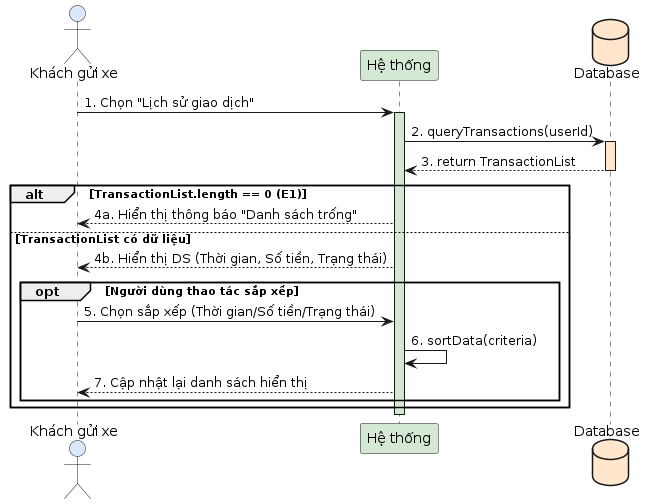
\includegraphics[width=0.8\textwidth]{pictures/seq_lichsugiaodich.png}
    \caption{Sequence diagram cho Use-case U3.1: Xem lịch sử giao dịch cá nhân}
\end{figure}

\begin{figure}[htbp]
    \centering
    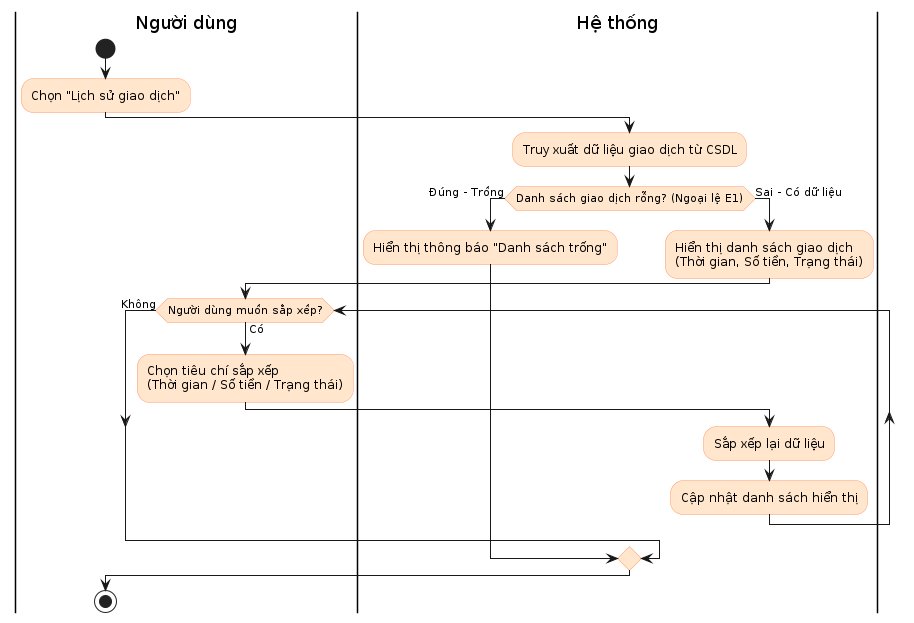
\includegraphics[width=0.8\textwidth]{pictures/lichsugiaodich.png}
    \caption{Activity diagram cho Use-case U3.1: Xem lịch sử giao dịch cá nhân}
\end{figure}

% --- Use Case U3.2 ---
\subsubsection{Use-case U3.2: Thanh toán hóa đơn}
\noindent
\begin{tabularx}{\textwidth}{|>{\raggedright\arraybackslash}p{4cm}|X|}
\hline
\textbf{Use-case ID} \newline \textbf{Use-case name} & U3.2 \newline \textbf{Thanh toán hóa đơn} \\ \hline
\textbf{Use-case overview} & Cho phép người dùng thanh toán hóa đơn gửi xe thông qua cổng thanh toán BKPay. \\ \hline
\textbf{Actors} & 1. Khách gửi xe có tài khoản. \newline 2. BKPay. \\ \hline
\textbf{Preconditions} & 
1. Hệ thống kết nối tới các máy chủ đã xác thực và khả dụng \newline
2. Người dùng đã đăng nhập \newline
3. Hệ thống đã tính toán phí gửi xe và gửi yêu cầu thanh toán lên BKPay \newline
4. Tồn tại hóa đơn chưa thanh toán. \\ \hline
\textbf{Trigger} & Người dùng chọn “Thanh toán hóa đơn” trên hệ thống. \\ \hline
\textbf{Steps} & 
1. Hệ thống hiển thị danh sách hóa đơn (gồm số tiền, thời hạn thanh toán).\newline
2. Người dùng chọn chuyển sang BKPay.\newline
3. BKPay hiển thị danh sách hóa đơn chưa thanh toán. \newline
4. Người dùng chọn ``Thanh toán'' trên một hóa đơn.\newline
5. Người dùng thanh toán trên BKPay.\newline
6. BKPay trả kết quả về hệ thống: 
\vspace*{-10pt}
    \begin{itemize}
        \item Thành công → cập nhật trạng thái “Đã thanh toán”.
        \vspace*{-10pt}
        \item Thất bại → ghi nhận “Chưa thanh toán”. 
    \end{itemize}
\vspace*{-10pt}
\\ \hline
\textbf{Post conditions} &  
                            1. Giao dịch được lưu vào lịch sử giao dịch. \newline
                            2. Người dùng nhận thông báo kết quả ``Giao dịch thành công''.
 \\ \hline
\textbf{Exception flow} & 
\textbf{E1 (Hết hạn thanh toán):} Gửi nhắc nhở 3 lần. Nếu vẫn chưa thanh toán thì khóa tài khoản. Dù tài khoản bị khóa không cho gửi xe nữa, nhưng hệ thống vẫn cho phép thanh toán để gỡ khóa.\\ \hline
\end{tabularx}

\vspace{0.5cm}
\begin{figure}[H]
    \centering
    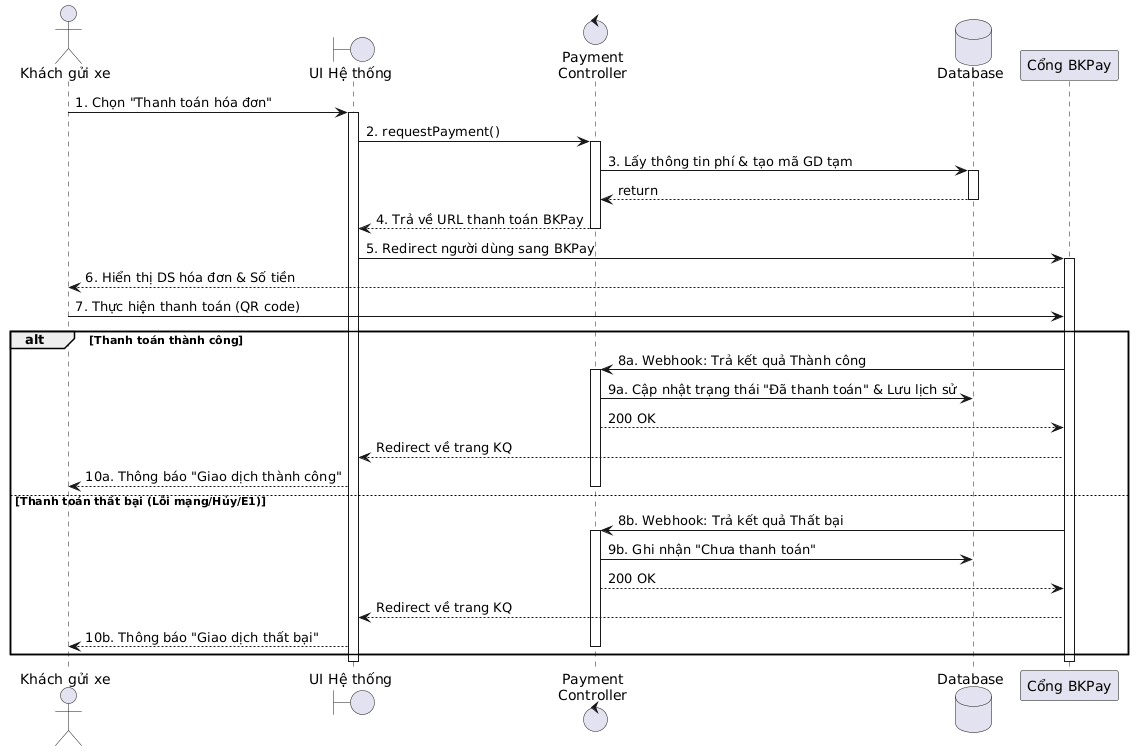
\includegraphics[width=0.7\textwidth]{pictures/seq_thanhtoanhoadon.png}
    \caption{Sequence diagram cho Use-case U3.2: Thanh toán hóa đơn}
\end{figure}

\begin{figure}[H]
    \centering
    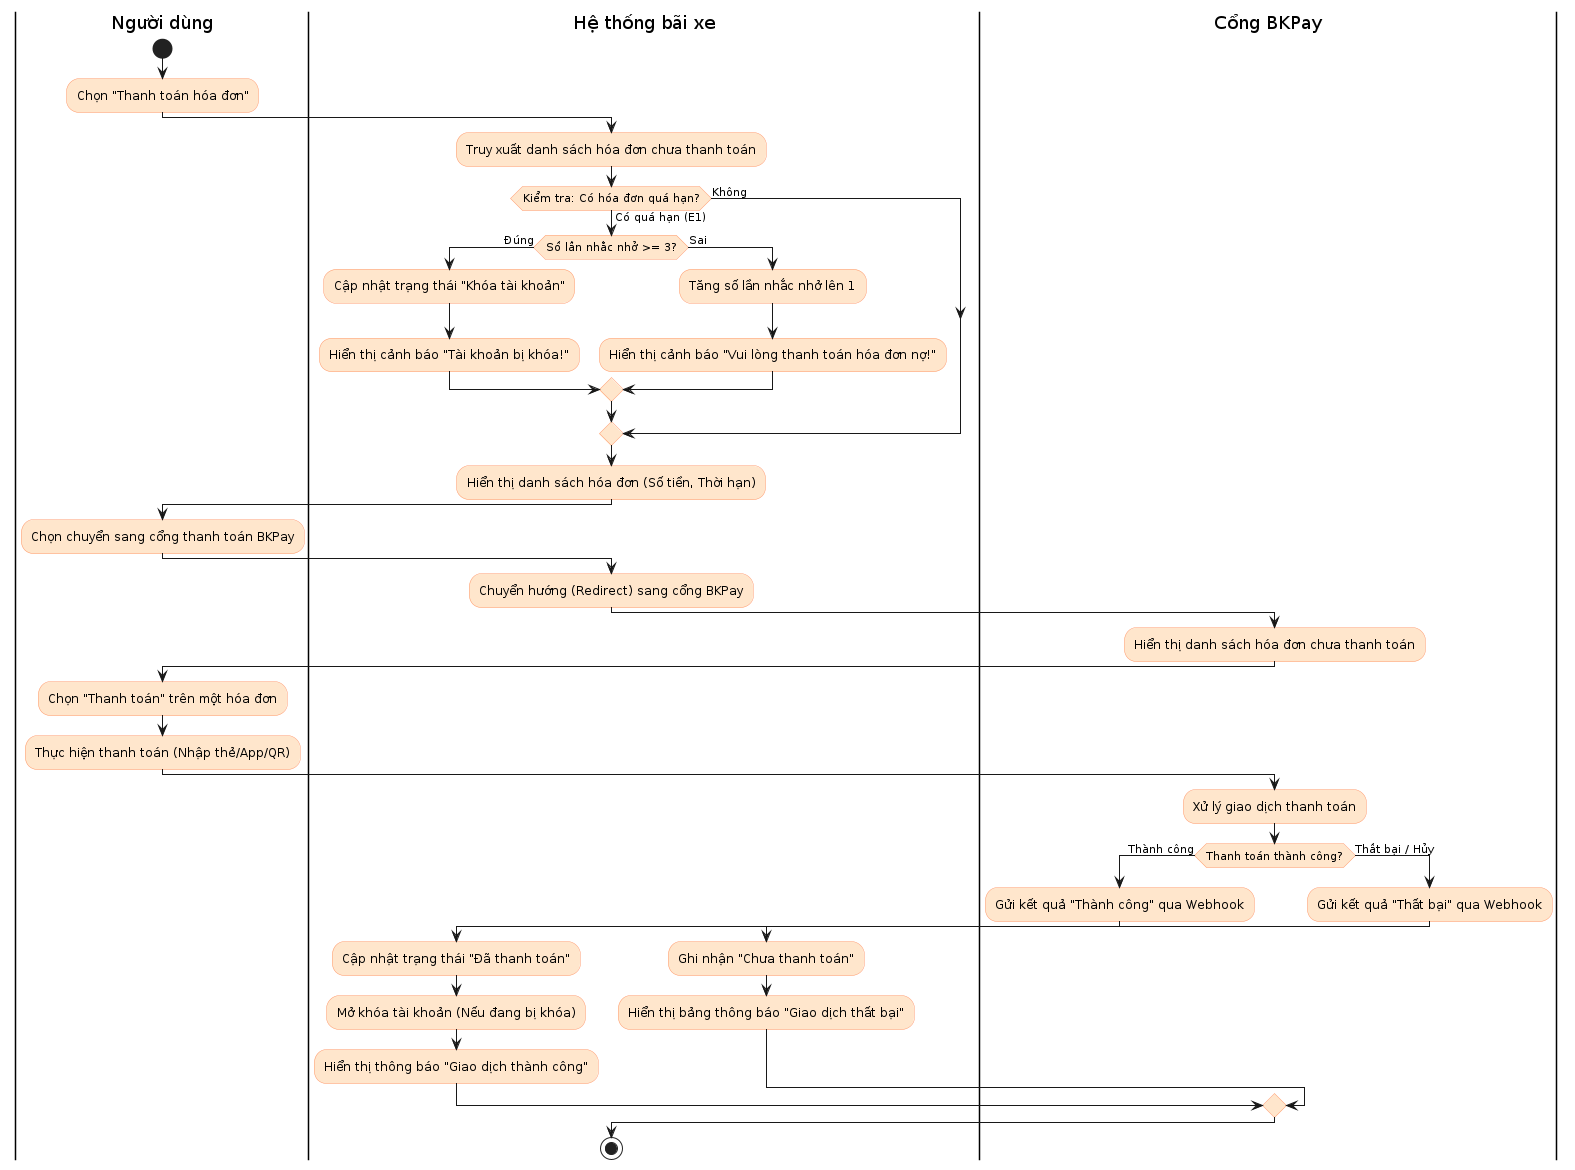
\includegraphics[width=0.7\textwidth]{pictures/thanhtoanhoadon.png}
    \caption{Activity diagram cho Use-case U3.2: Thanh toán hóa đơn}
\end{figure}

% --- Use Case U3.3 ---
\subsubsection{Use-case U3.3: Thanh toán thủ công}
\noindent
\begin{tabularx}{\textwidth}{|>{\raggedright\arraybackslash}p{4cm}|X|}
\hline
\textbf{Use-case ID} \newline \textbf{Use-case name} & U3.3 \newline \textbf{Thanh toán thủ công} \\ \hline
\textbf{Use-case overview} & Cho phép thanh toán thủ công, hỗ trợ bởi nhân viên bãi xe. \\ \hline
\textbf{Actors} & 1. Khách gửi xe có tài khoản hoặc không có tài khoản. \newline
                    2. Nhân viên bãi xe\\ \hline
\textbf{Preconditions} & 
1. Người gửi xe chọn thanh toán thủ công khi vào cổng và được phát thẻ tạm.\newline
2. Hệ thống ghi nhận giao dịch, biển số xe và thời gian bắt đầu gửi xe.\newline
2. Hệ thống đã tính được phí gửi xe.
\\ \hline
\textbf{Trigger} & Người gửi xe có mặt tại cổng ra. \\ \hline
\textbf{Steps} & 
1. Người gửi xe sử dụng thẻ tạm để quét vào hệ thống.\newline
2. Hệ thống truy xuất phiên gửi xe và tính phí từ cơ sở dữ liệu.\newline
3. Hệ thống hiển thị số tiền cần trả cho cả người gửi xe và nhân viên bãi xe nhìn thấy.\newline
4. Người gửi xe trả tiền mặt (vật lý) cho nhân viên.\newline
5. Nhân viên bấm ``Xác nhận đã nhận tiền'' trên hệ thống.\newline
6. Hệ thống đánh dấu giao dịch ``Đã thanh toán'' vào cơ sở dữ liệu.\newline
7. Hệ thống ra lệnh mở barie, cho phép xe rời bãi.
 \\ \hline
\textbf{Post conditions} & 1. Giao dịch được đánh dấu đã thanh toán. \newline
                            2. Xe được phép rời bãi.

 \\ \hline
\textbf{Exception flow} & 
- \textbf{E1 (Thẻ bị lỗi / Không tìm thấy giao dịch):} Xảy ra ở bước 2 nếu CSDL không tìm thấy thông tin hoặc thẻ hỏng. Hệ thống báo lỗi. 
                                Nhân viên hỏi thông tin (biển số/giấy tờ) của khách và nhập dữ liệu xác minh thủ công. Hệ thống tạo lập giao dịch thủ công. Chuyển sang bước thanh toán và mở barie. \newline
- \textbf{E2 (Khách mất thẻ):} Khách không thể thực hiện bước 1. Khách báo mất thẻ cho nhân viên. Nhân viên hỏi thông tin (biển số/giấy tờ) và nhập xác minh ``báo mất thẻ'' lên hệ thống. 
                        Hệ thống tạo giao dịch thủ công và tính cộng thêm phí phạt. Khách trả tiền và nhân viên mở barie.
 \\ \hline
\end{tabularx}

\vspace{0.5cm}

\begin{figure}[htbp]
    \centering
    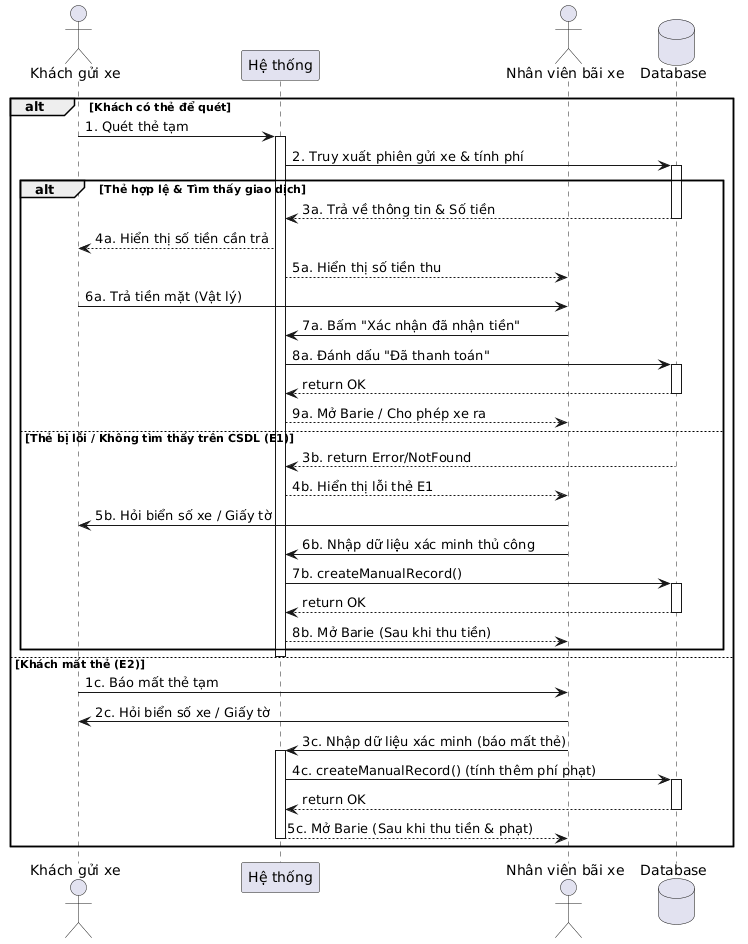
\includegraphics[width=0.8\textwidth]{pictures/seq_thanhtoanthucong.png}
    \caption{Sequence diagram cho Use-case U3.3: Thanh toán thủ công}
\end{figure}

\begin{figure}[htbp]
    \centering
    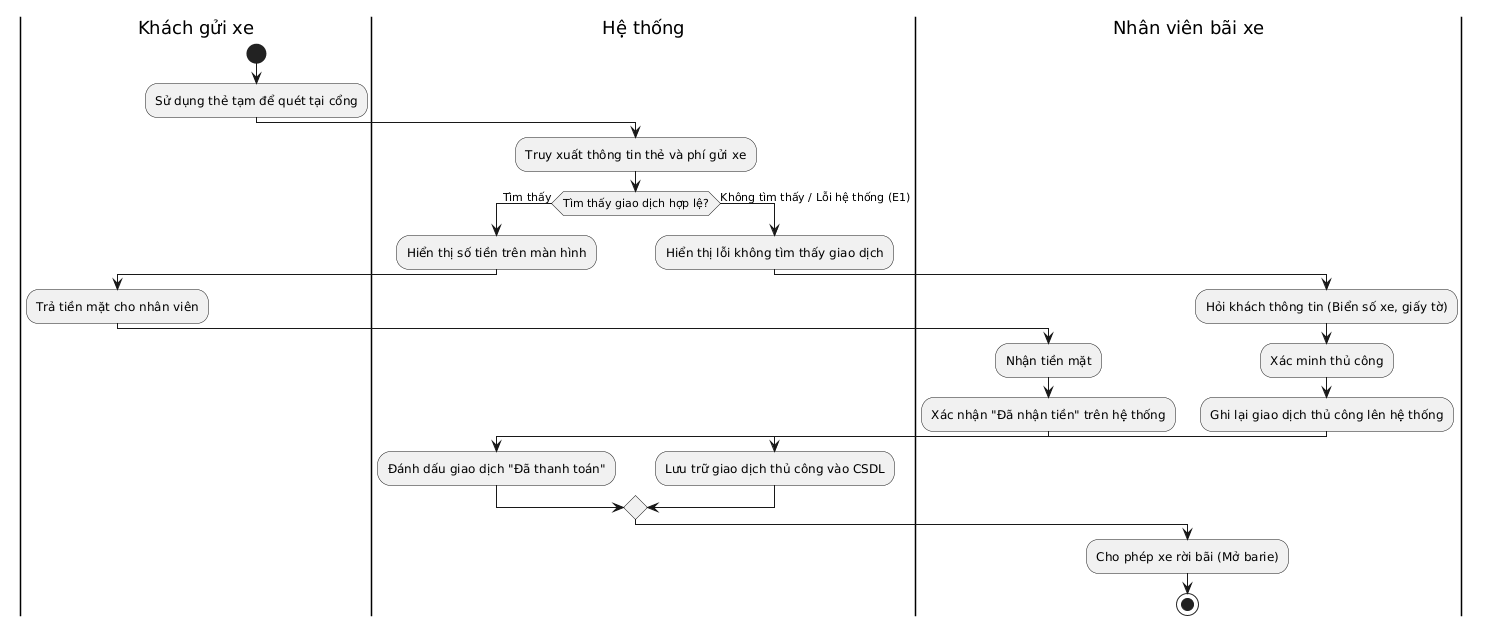
\includegraphics[width=0.8\textwidth]{pictures/thanhtoanthucong.png}
    \caption{Activity diagram cho Use-case U3.3: Thanh toán thủ công}
\end{figure}
\newpage
